

\documentclass{beamer}

\mode<presentation> {

% The Beamer class comes with a number of default slide themes
% which change the colors and layouts of slides. Below this is a list
% of all the themes, uncomment each in turn to see what they look like.


\usetheme{Boadilla}



\setbeamertemplate{footline}  


}
\setbeamersize{text margin left=1cm, }
\setbeamertemplate{frametitle}[default][center]
\usepackage{graphicx} 
\usepackage{booktabs} 

	\usepackage{changepage}


\usepackage{cite}
\usepackage{setspace}
\usepackage{color}
\usepackage[normalem]{ulem}
\newtheorem{hyp}{Hypothesis}


\usepackage{epsfig}
\usepackage{amsmath}
\usepackage{amssymb}
\usepackage{multicol}
\usepackage{amsmath, amsthm, amssymb}


\usepackage{graphicx}
\usepackage{tikz}
\usetikzlibrary{shapes,arrows}
\usepackage{tikz}
\usepackage{amsmath, amsthm, amssymb}
%----------------------------------------------------------------------------------------
%	TITLE PAGE
%----------------------------------------------------------------------------------------



\begin{document}
	

  

\begin{frame}
	\frametitle{Web Data -- Twitter}
	\pause 

\end{frame}



\begin{frame}
	\centering Why should we care about social media? \vspace{.5cm}
	\begin{enumerate}
		\item<2> Social media usage is widespread
	\end{enumerate}
	
\end{frame}


%
\begin{frame}
	Widespread use of social media sites\vspace{.7cm}\\
	\begin{minipage}[0.2\textheight]{\textwidth}
		\begin{columns}[T]
			\begin{column}{0.7\textwidth}
				\begin{itemize}[<+->]
					\item One in every ten people in the world logged onto Facebook yesterday.
					\item 71\% of online adults in the US use Facebook (84\% use among ages 18--29)
					\item 400+ million tweets are sent everyday by 200+ million active users worldwide
					\item 23\% of online adults in the US use Twitter (31\% use among ages 18--29)\\
					\item Instagram has 300+ million active users (26\% of online adults in the US)\\
				\end{itemize}
			\end{column}
			\begin{column}{0.2\textwidth}
				\vspace{.25cm}
				
\includegraphics[width=1.8cm]{figures/facebook_logo.png}\\ \vspace{.2cm}
				\uncover<3->{
\includegraphics[width=1.8cm]{figures/twitter_logo.png}}\\ \vspace{.2cm}
				\uncover<5->{
\includegraphics[width=1.8cm]{figures/Instagram_Icon_Large}}
			\end{column}
		\end{columns}
	\end{minipage}
	\vfill
	\hfill\tiny{(Sources: Pew Research Center (2014), Twitter and Facebook official statistics)}
	
\end{frame}

\begin{frame}
	\centering Why should we care about social media? \vspace{.5cm}
	\begin{enumerate}
		\item Social media usage is widespread
		\item Social media usage is increasing
		
	\end{enumerate}
	
\end{frame}


\begin{frame}
	\frametitle{Social media usage is increasing}
	\begin{figure} 
		\includegraphics<1>[width=.9\textwidth]{figures/users_by_country_1.pdf}
		
		\includegraphics<2>[width=.9\textwidth]{figures/users_by_country_2.pdf}
		
		\includegraphics<3>[width=.9\textwidth]{figures/users_by_country_3.pdf}
	\end{figure}
	
	\vfill
	\hfill\tiny{(Source: Zeitzoff and Barber\'{a}, ISQ 2017)}
	
\end{frame}

\begin{frame}
	\centering Why should we care about social media? \vspace{.5cm}
	\begin{enumerate}
		\item Social media usage is widespread
		\item Social media usage is increasing
		\item Political content on social media
	\end{enumerate}
	
\end{frame}


\begin{frame}
	Social media and politics
	\begin{itemize}[<+->]
		\item 99\% of Members of the US Congress have an active social media account
		\item 80\% of governments have a presence on Twitter
		\item ``Traditional'' media outlets rely on social media to promote their content
		\item 50\% of social media users in U.S. share information about news stories, images or videos about current events
		\item 46\% have discussed a news issue or event on social media
	\end{itemize}
	
	\vfill
	\hfill\tiny{(Sources: Electionista; Zeitzoff and Barber\'{a}, ISQ 2017; Pew Research Center)}
	
\end{frame}

\begin{frame}
	
	Social media as a new campaign tool:\\
	\vspace{.05cm} \begin{footnotesize}
		\begin{quote}\indent ``Let me tell you about Twitter. I think that maybe I wouldn't be here if it wasn't for Twitter. [...] Twitter is a wonderful thing for me, because I get the word out... I might not be here talking to you right now as president if I didn't have an honest way of getting the word out.'' \\
			\vspace{.1cm}
			\hfill \textbf{Donald Trump}, \textit{March 16, 2017} (Fox News) \end{quote}\end{footnotesize}
	\pause
	\begin{itemize}[<+->]
		\item Diminished \alert{gatekeeping} role of journalists
		\begin{itemize}
			\item \scriptsize{Part of a trend towards citizen journalism (Goode, 2009)}
		\end{itemize}
		\item Information is contextualized within \alert{social layer}
		\begin{itemize}
			\item  \scriptsize{Messing and Westwood (2012): social cues can be as important as partisan cues to explain news consumption through social media}
		\end{itemize}
		\item \alert{Real-time broadcasting} in reaction to events
		\begin{itemize}
			\item  \scriptsize{e.g. \textit{dual screening} (Vaccari et al, 2015)}
		\end{itemize}
		\item \alert{Micro-targeting}
		\begin{itemize}
			\item  \scriptsize{Affects how campaigns perceive voters (Hersh, 2015), but unclear if effective in mobilizing or persuading voters}
		\end{itemize}
	\end{itemize}
	
\end{frame}


\begin{frame}
	\centering Why should we care about social media? \vspace{.5cm}
	\begin{enumerate}
		\item Social media usage is widespread
		\item Social media usage is increasing
		\item Political content on social media
		\item Social media is a primary source of political information
	\end{enumerate}
\end{frame}


\begin{frame}
	\frametitle{Social media research}
	
	Two different approaches to the study of social media and politics:\vspace{.5cm}
	\begin{enumerate}
		\item Social media as a new source of information
		\begin{itemize}
			\item Behavior, opinions, and latent traits
			\item Interpersonal networks
			\item Elite behavior
		\end{itemize}
		\item How social media usage affect social behavior
		\begin{itemize}
			\item Mass protests
			\item Political persuasion
			\item Social capital
			\item Political polarization
		\end{itemize}
	\end{enumerate}
\end{frame}


\begin{frame}
	\frametitle{Social media as echo chambers?}
	
	\vspace{.2cm}
	\begin{itemize} 
		\item communities of like-minded individuals (homophily, influence)
	\end{itemize}
	
	\begin{figure}
		\begin{tabular}{cc}
			\hspace{-.5cm}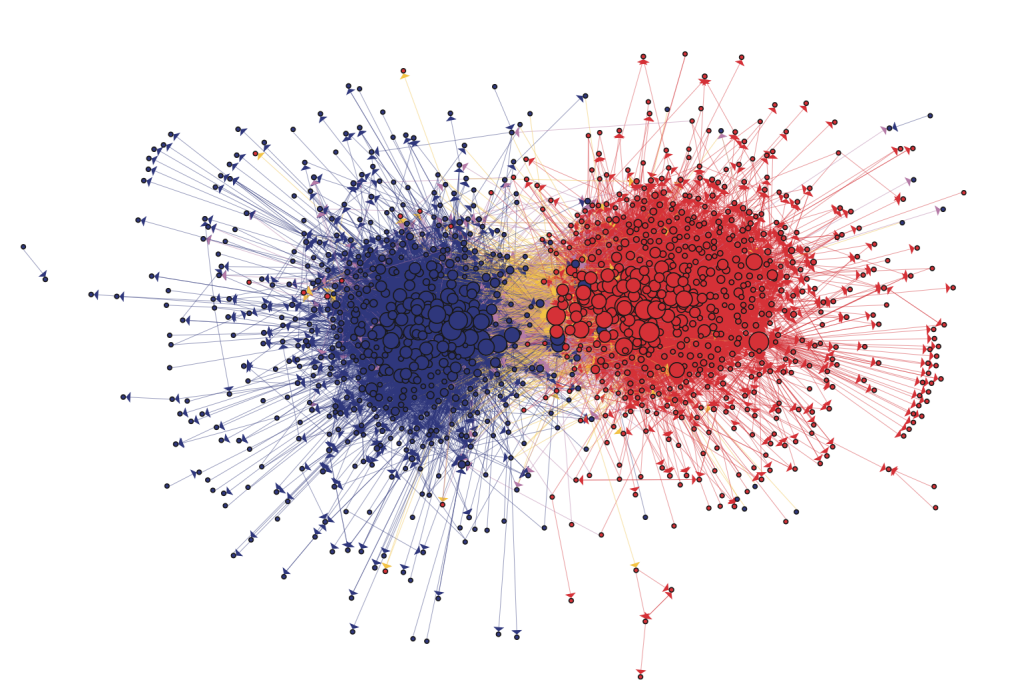
\includegraphics[width=.40\textwidth]{figures/adamic.png} &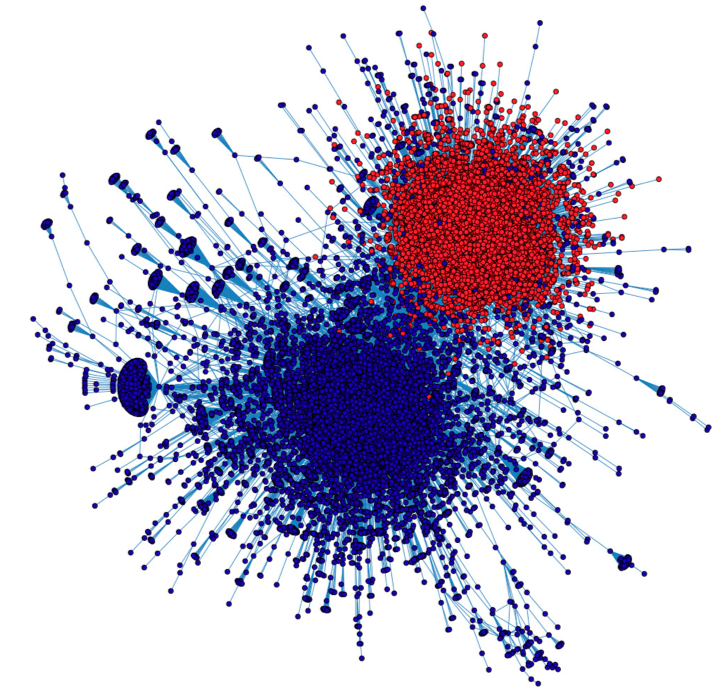
\includegraphics[width=.40\textwidth]{figures/conover} \\
			\tiny{Adamic and Glance (2005)} & \tiny{Conover et al (2012)} \\
		\end{tabular}
	\end{figure}
	
	\vspace{.2cm}
	\uncover<2->{\begin{itemize}[<+->]
			\item ...generates selective exposure to congenial information
			\item ...reinforced by ranking algorithms -- ``filter bubble'' (Parisier)
			\item ...increases political polarization (Sunstein, Prior)
	\end{itemize}}
\end{frame}


\setlength{\leftmargini}{6pt}
\begin{frame}
	\frametitle{Social media as echo chambers?}
	
	\begin{figure}
		\begin{tabular}{cc}
			\hspace{-.5cm}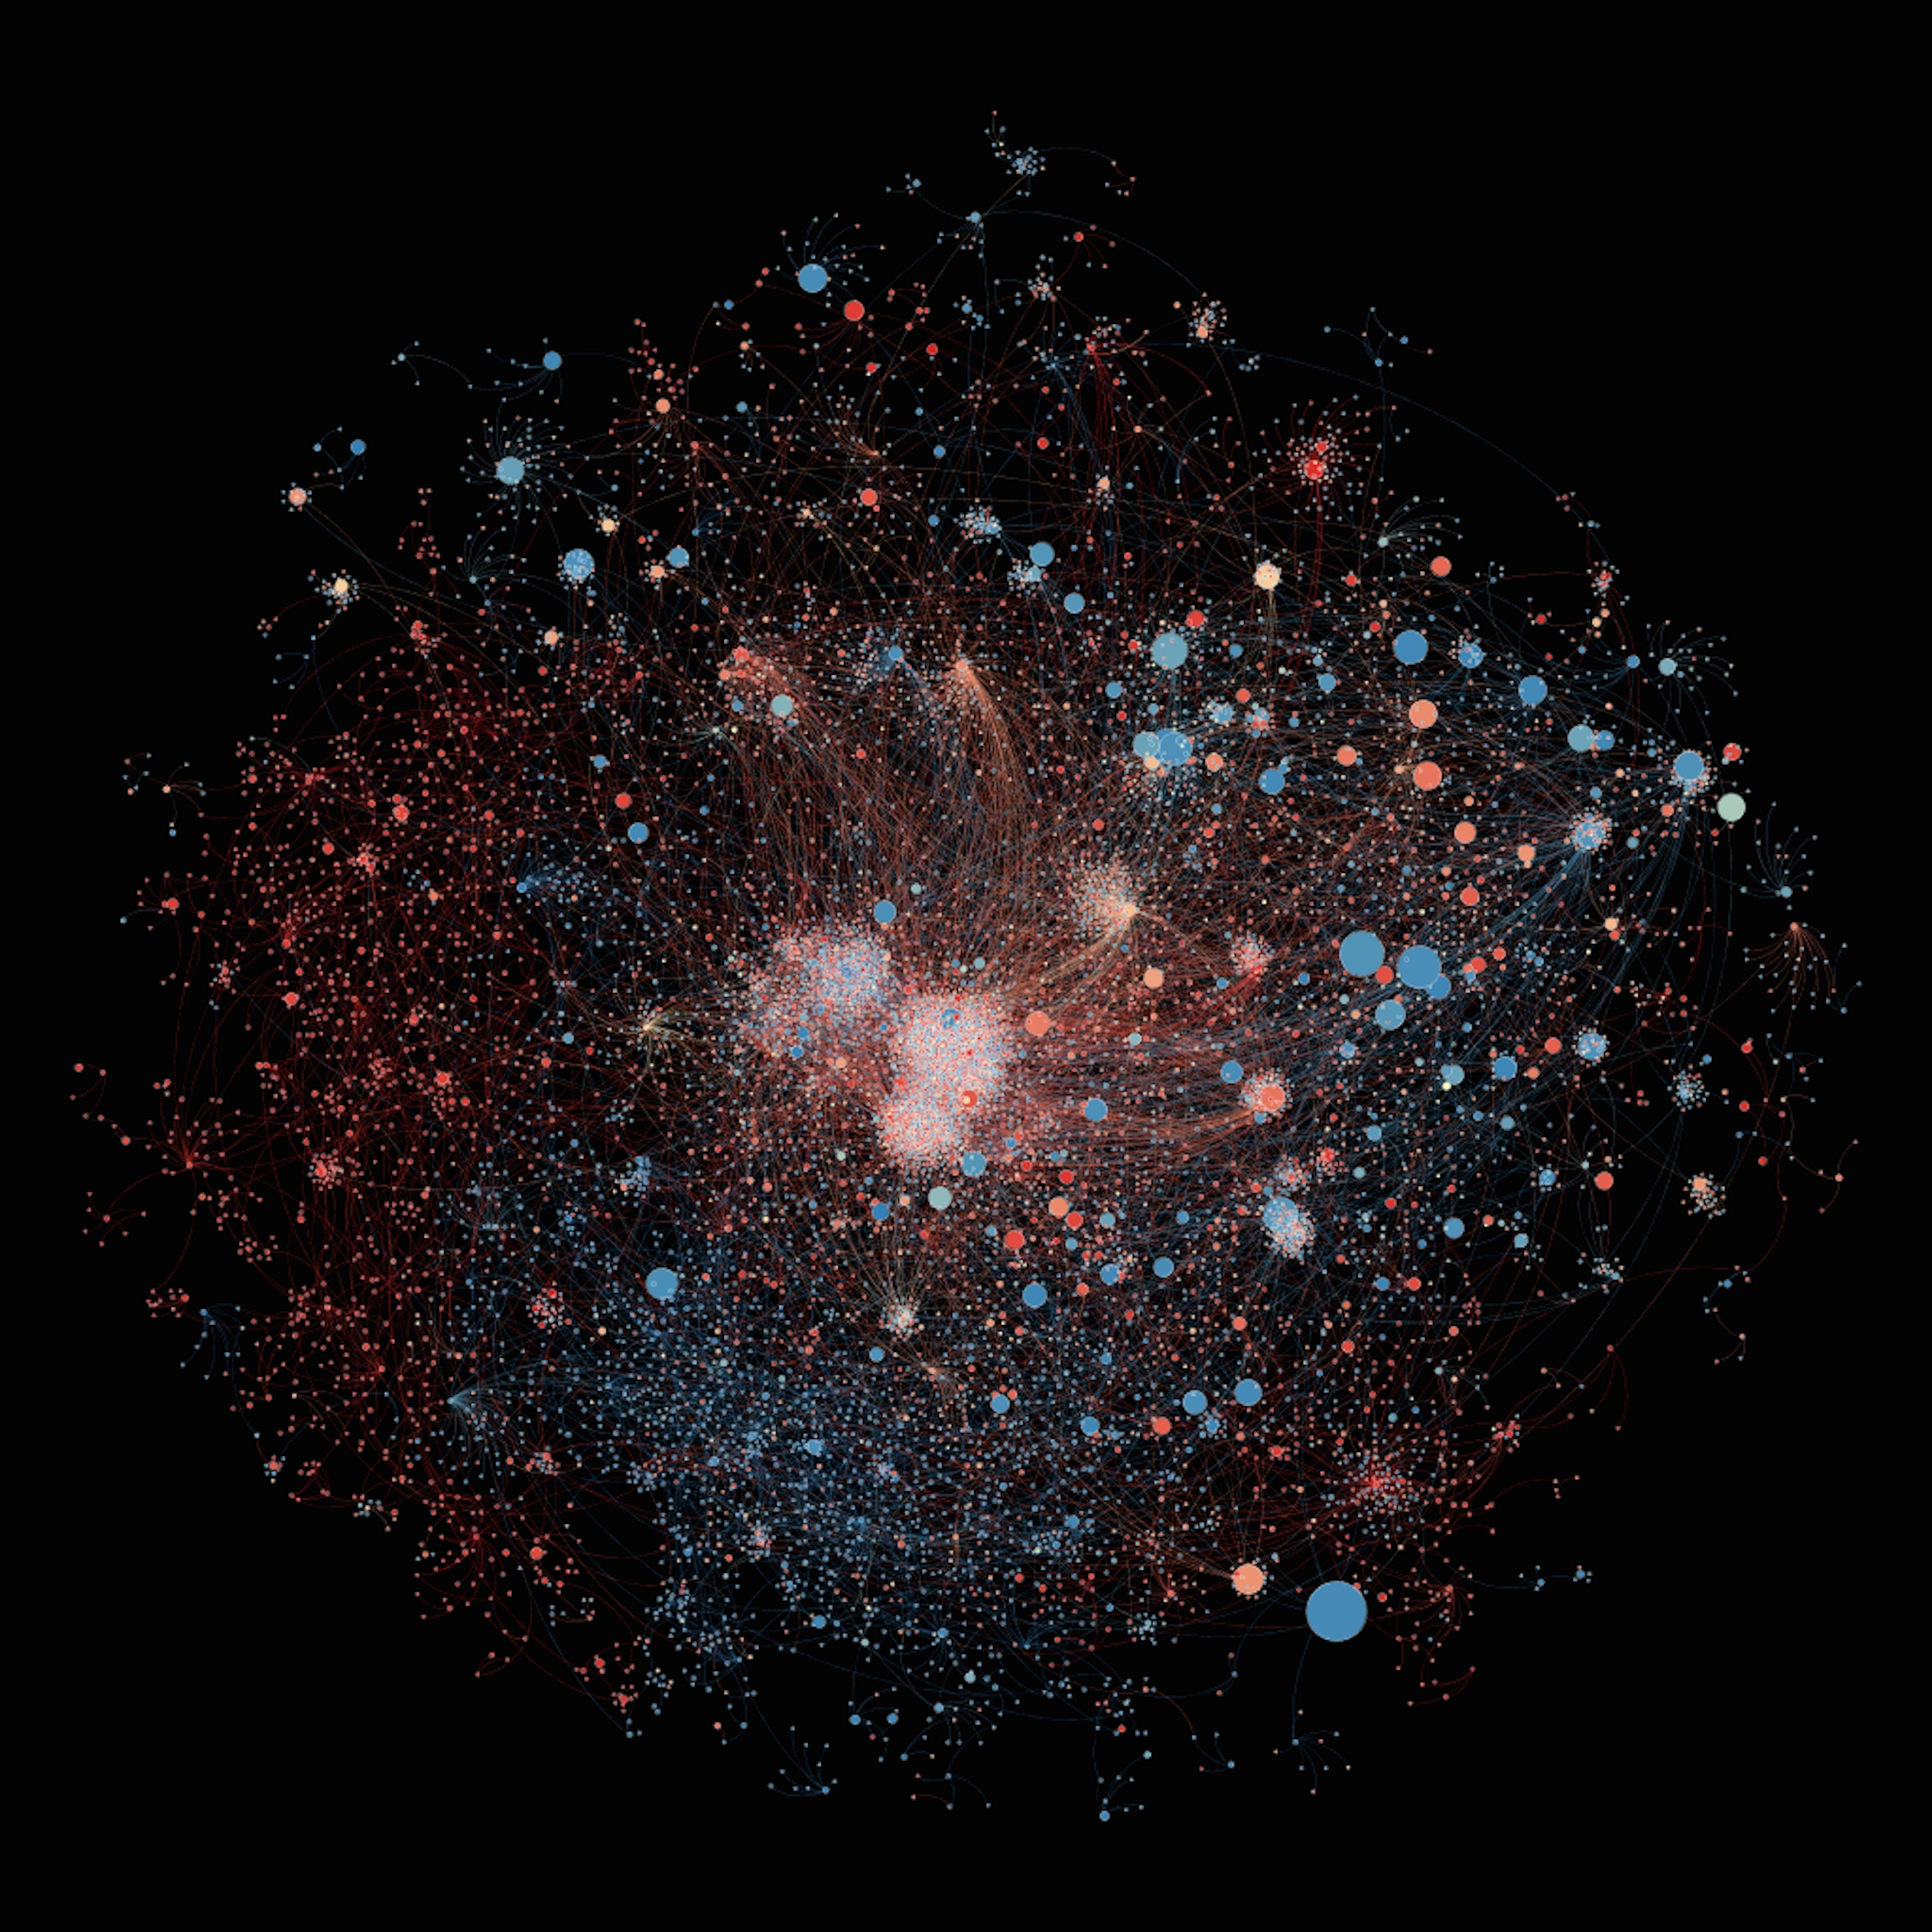
\includegraphics[width=.45\textwidth]{figures/figure3b.jpg} & 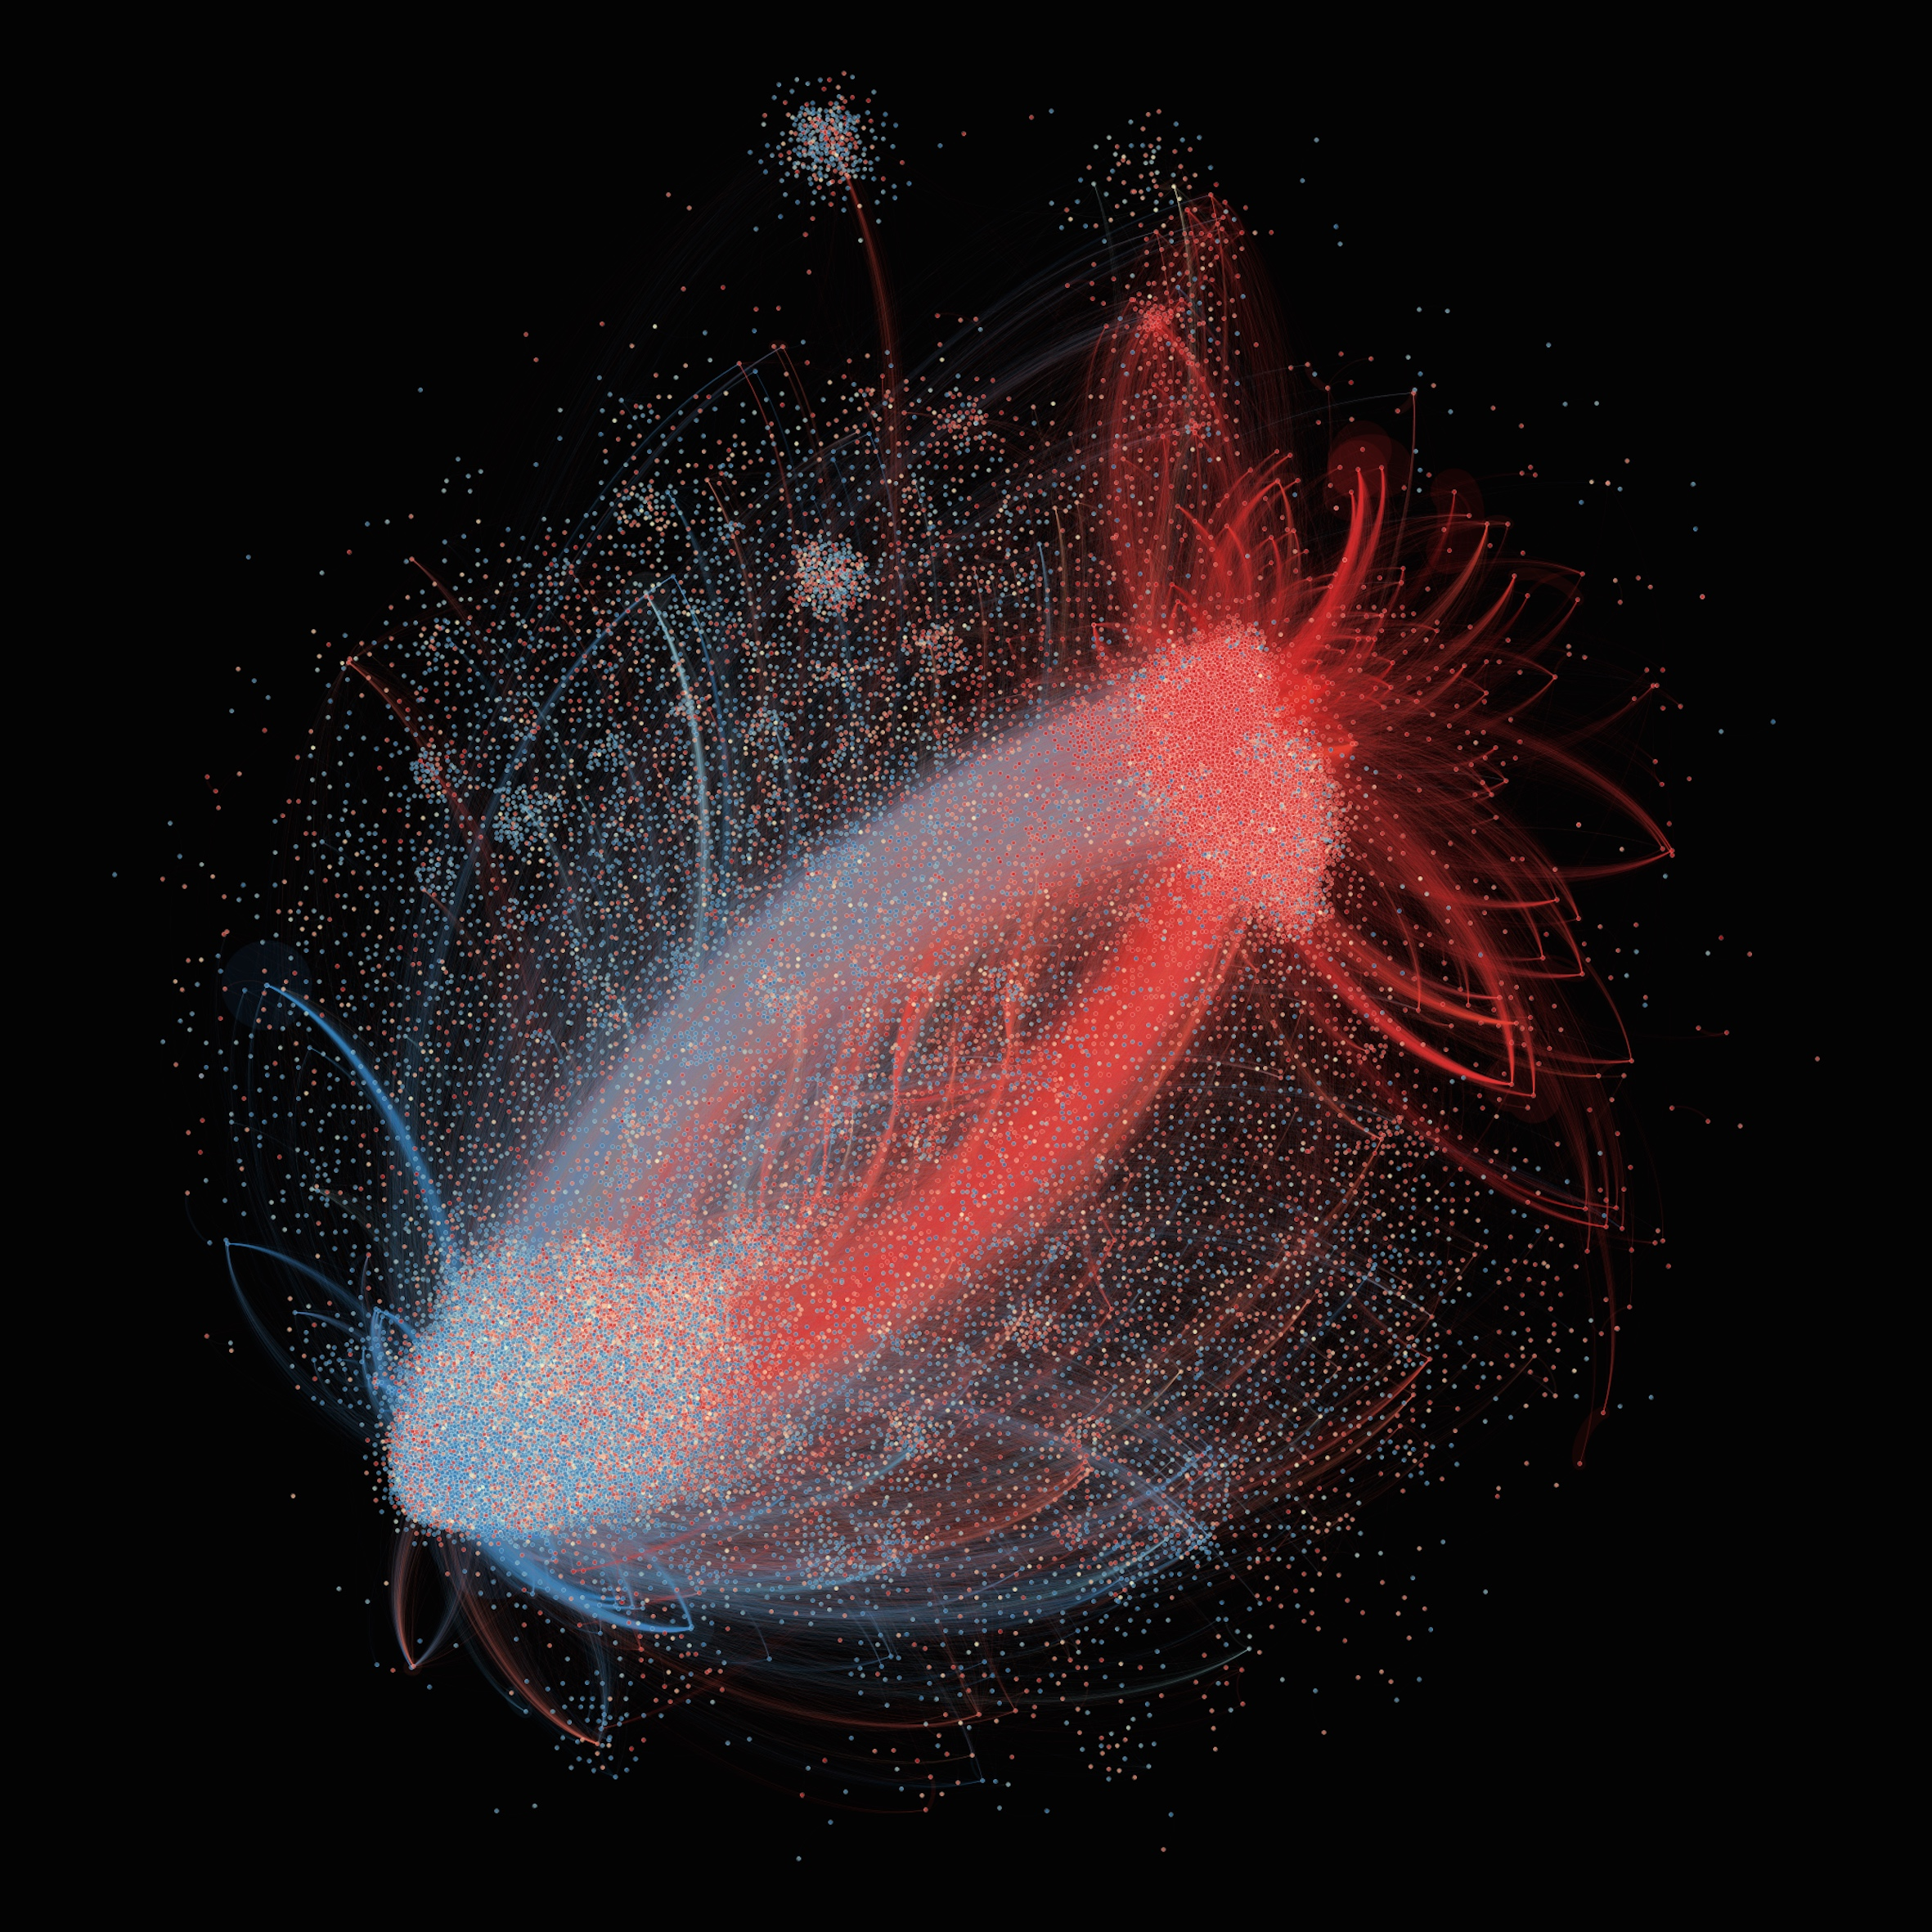
\includegraphics[width=.45\textwidth]{figures/figure3a.jpg}\\
			\small{2013 SuperBowl}  & \small{2012 Election} \\
		\end{tabular}
	\end{figure}
	
	\vspace{.10cm}
	\vfill
	\footnotesize{Barber\'{a} et al (2015) ``Tweeting From Left to Right: Is Online Political Communication More Than an Echo Chamber?'' \textit{Psychological Science}}
\end{frame}
\setlength{\leftmargini}{12pt}

\begin{frame}
	\frametitle{Social media as echo chambers?}
	
	\hspace{-.75cm}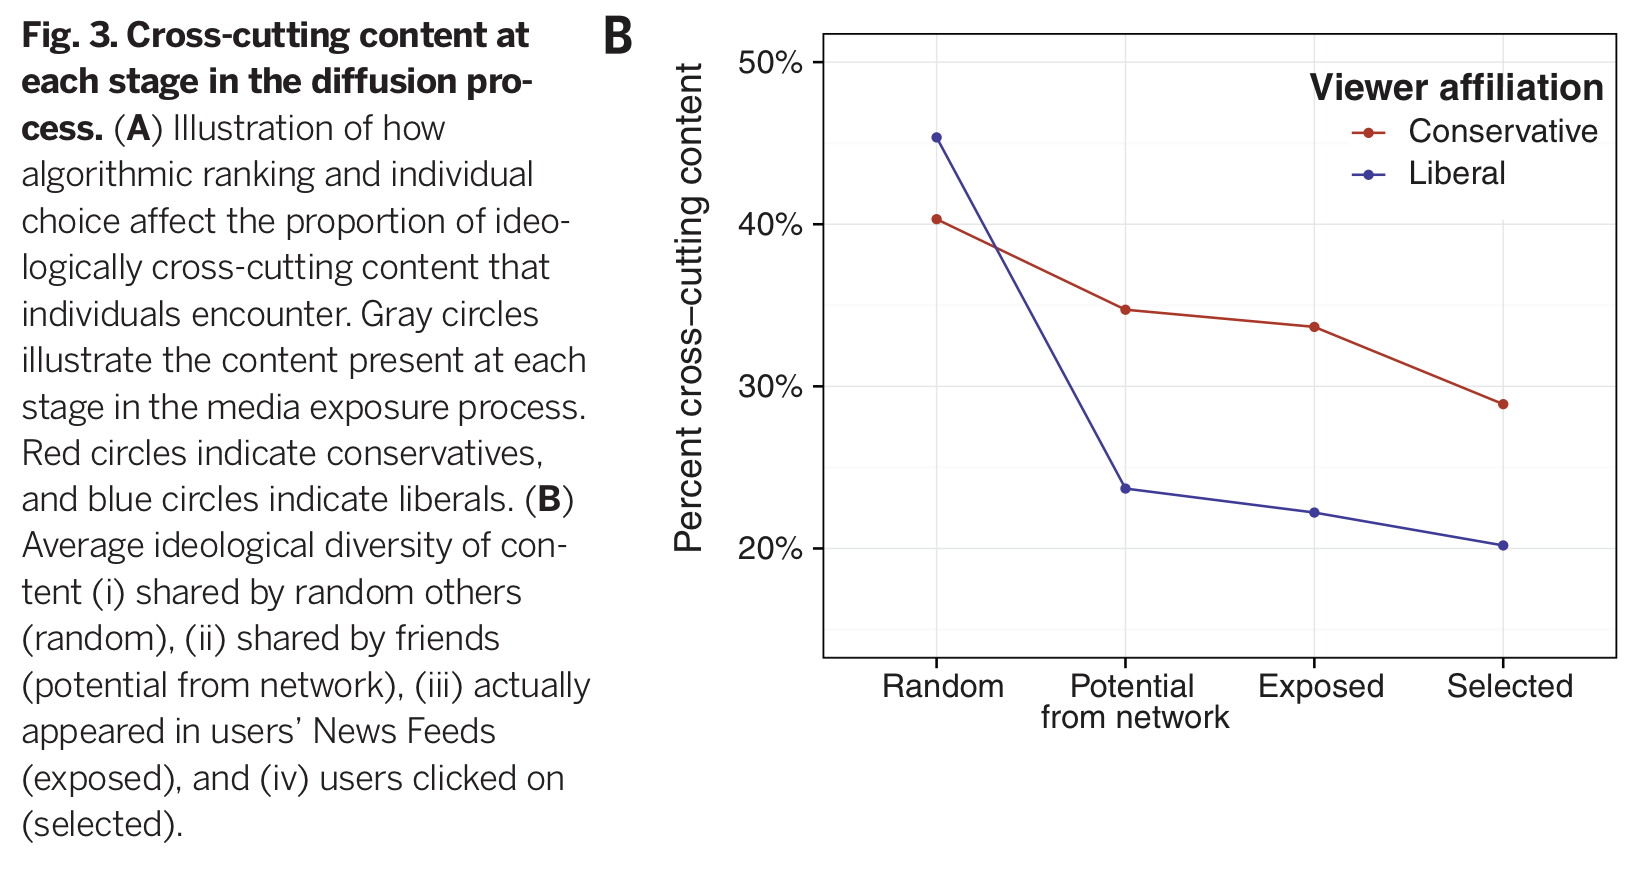
\includegraphics[width=.9\paperwidth]{figures/messing-science.png}\\
	
	\vspace{.10cm}
	\small{Bakshy, Messing, \& Adamic (2015) ``Exposure to ideologically diverse news and opinion on Facebook''. \textit{Science.}}
\end{frame}

\begin{frame}
	
	\centering\Huge{Twitter data}
	
\end{frame}



\begin{frame}
	\frametitle{Twitter APIs}
	Two different methods to collect Twitter data:
	\begin{enumerate}[<+->]
		\item REST API:
		\begin{itemize}
			\item Queries for specific information about users and tweets
			\item Search recent tweets
			\item Examples: user profile, list of followers and friends, tweets generated by a given user (``timeline''), users lists, etc.
			\item R library: netdemR (also twitteR, rtweet)
		\end{itemize}
		\item Streaming API:
		\begin{itemize}
			\item Connect to the ``stream'' of tweets as they are being published
			\item Three streaming APIs:
			\begin{enumerate}
				\item Filter stream: tweets filtered by keywords
				\item Geo stream: tweets filtered by location
				\item Sample stream: 1\% random sample of tweets
			\end{enumerate}
			\item R library: streamR
		\end{itemize}
	\end{enumerate}
	\uncover<+->{\alert{Important limitation:} tweets can only be downloaded in real time (exception: user timelines, $\sim$ 3,200 most recent tweets are available)}
	
\end{frame}

\begin{frame}
	\frametitle{Anatomy of a tweet}
	\centering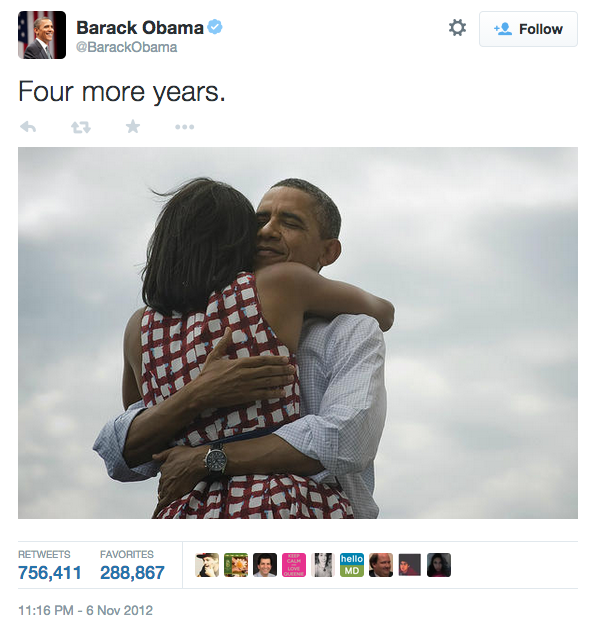
\includegraphics[height=.8\textheight]{figures/obama.png}
	
\end{frame}

\begin{frame}[fragile]
	\frametitle{Anatomy of a tweet}
	Tweets are stored in JSON format:\vspace{.25cm}\\
	\centering\begin{minipage}[c]{.80\textwidth}
		\begin{tiny}\begin{verbatim}
			{ "created_at": "Wed Nov 07 04:16:18 +0000 2012",
			"id": 266031293945503744,
			"text": "Four more years. http://t.co/bAJE6Vom",
			"source": "web",
			"user": {
			"id": 813286,
			"name": "Barack Obama",
			"screen_name": "BarackObama",
			"location": "Washington, DC",
			"description": "This account is run by Organizing for Action staff. 
			Tweets from the President are signed -bo.",
			"url": "http://t.co/8aJ56Jcemr",
			"protected": false,
			"followers_count": 54873124,
			"friends_count": 654580,
			"listed_count": 202495,
			"created_at": "Mon Mar 05 22:08:25 +0000 2007",
			"time_zone": "Eastern Time (US & Canada)",
			"statuses_count": 10687,
			"lang": "en" },
			"coordinates": null,
			"retweet_count": 756411,
			"favorite_count": 288867,
			"lang": "en"
			}
			\end{verbatim}\end{tiny}\end{minipage}
\end{frame}


\begin{frame}
	\frametitle{Streaming API}
	\begin{itemize}[<+->]
		\item Recommended method to collect tweets
		\item Potential issues:
		\begin{itemize}
			\item Filter streams have same rate limit as spritzer: when volume reaches 1\% of all tweets, it will return random sample
			\item Stream connections tend to die spontaneously. Restart regularly.
			\item Lots of invalid content in stream. If it can't be parsed, drop it.
		\end{itemize}
		\item My workflow:
		\begin{itemize}
			\item Amazon EC2, cloud computing
			\item Cron jobs to restart R scripts every hour.
			\item Save tweets in .json files, one per day.

		\end{itemize}
	\end{itemize}
\end{frame}


\begin{frame}
	\frametitle{Sampling bias?}
	
	\alert{Morstatter} et al, 2013, \textit{ICWSM}, ``Is the Sample Good Enough? Comparing Data from Twitter's Streaming API with Twitter's Firehose'':
	\begin{itemize}
		\item 1\% random sample from Streaming API is not truly random
		\item Less popular hashtags, users, topics... less likely to be sampled
		\item But for keyword-based samples, bias is not as important
	\end{itemize}
	\pause
	
	\alert{Gonz\'{a}lez-Bail\'{o}n} et al, 2014, \textit{Social Networks}, ``Assessing the bias in samples of large online networks'':
	\begin{itemize}
		\item Small samples collected by filtering with a subset of relevant hashtags can be biased
		\item Central, most active users are more likely to be sampled
		\item Data collected via search (REST) API more biased than those collected with Streaming API
		
	\end{itemize}
	
	
	
\end{frame}


\begin{frame}
	
	\begin{columns}
		\column{1.7in}
		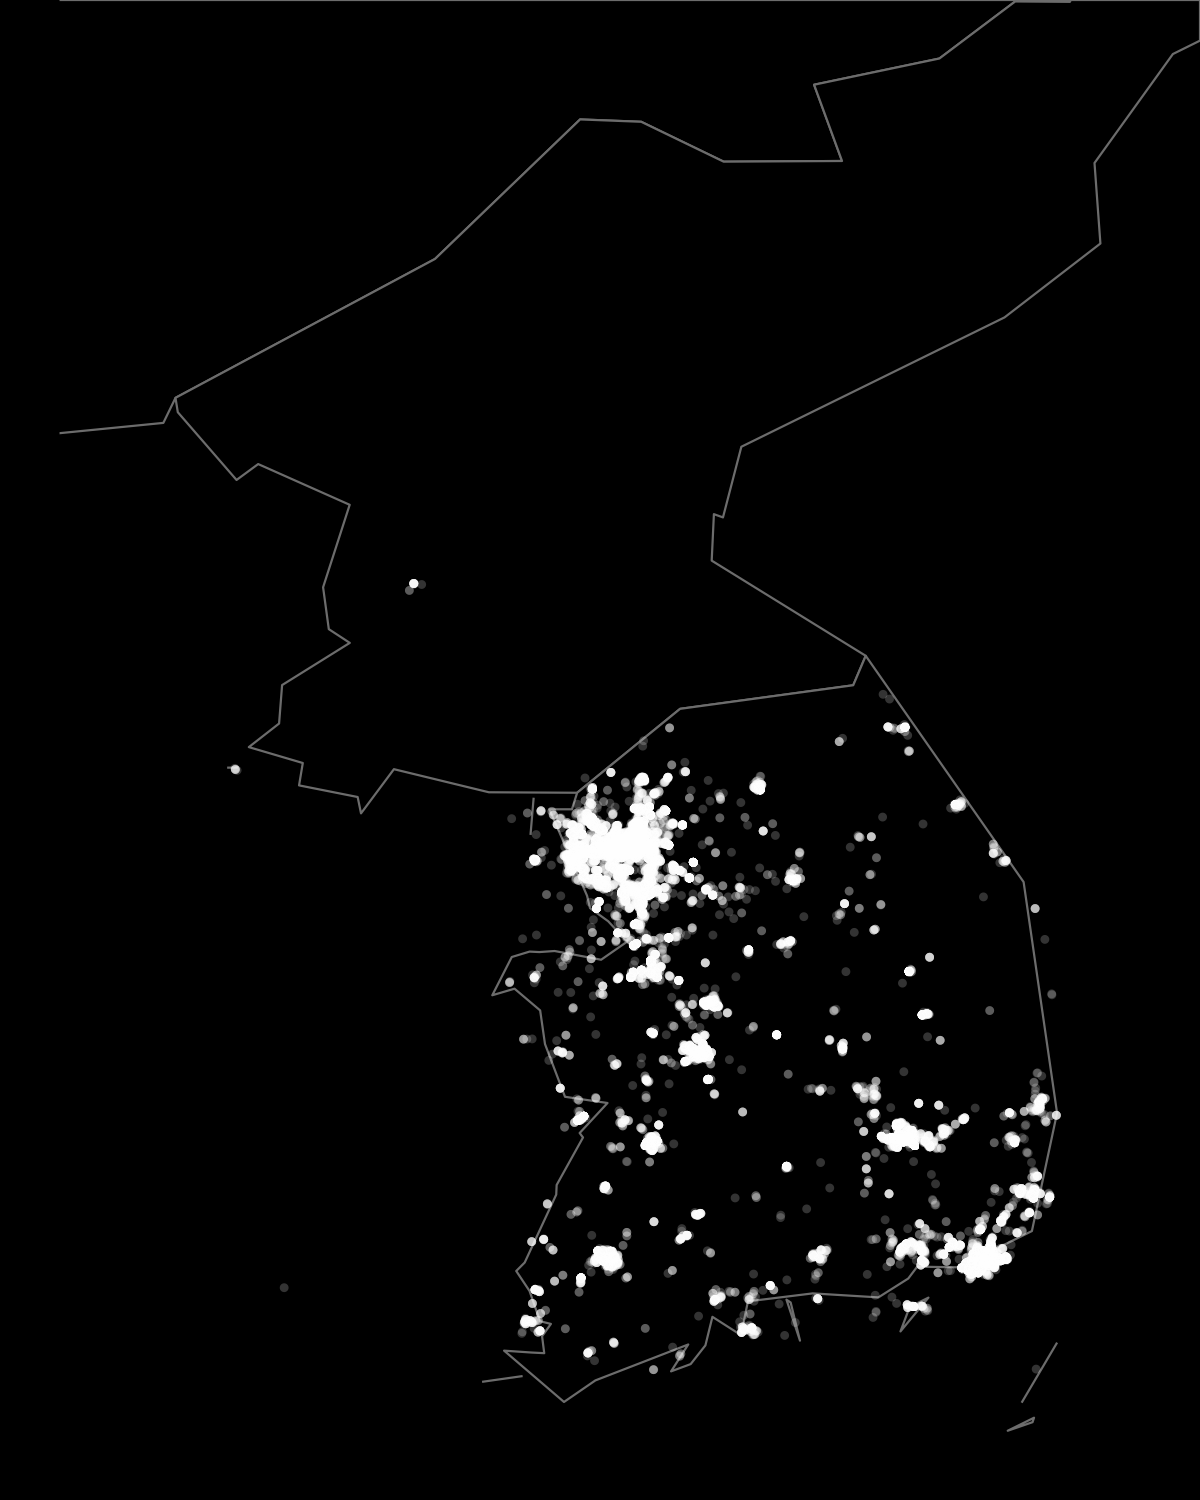
\includegraphics[width=1.2\textwidth]{figures/tweets_korea.png}
		\column{1.7in}
		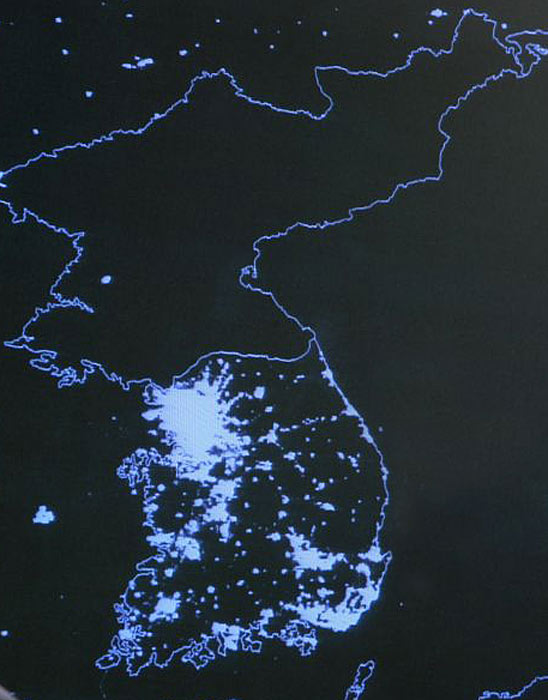
\includegraphics[width=1.2\textwidth]{figures/korea_lights.jpg}
	\end{columns}
	
	\begin{center}
		Tweets from Korea: 40k tweets collected in 2014 (left)\\
		Korean peninsula at night, 2003 (right). Source: NASA.
	\end{center}
	
	
\end{frame}

\begin{frame}[fragile]
	\frametitle{Who is tweeting from North Korea?}
	\begin{center}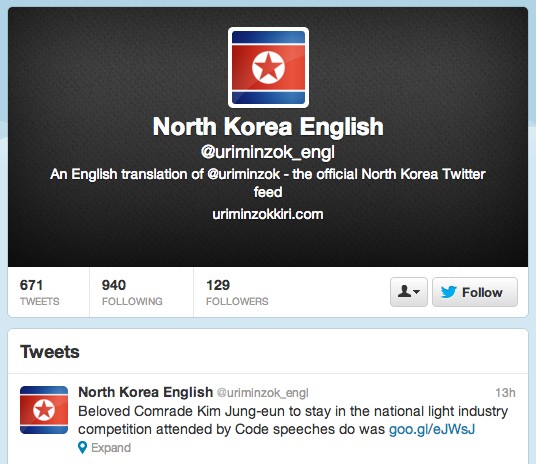
\includegraphics[width=.8\textheight]{figures/north_korea_tweet.png}\\
		Twitter user: \href{https://twitter.com/uriminzok_engl}{@uriminzok\_engl}\end{center}
\end{frame}


\begin{frame}[fragile]
	\frametitle{But remember...}
	\begin{center}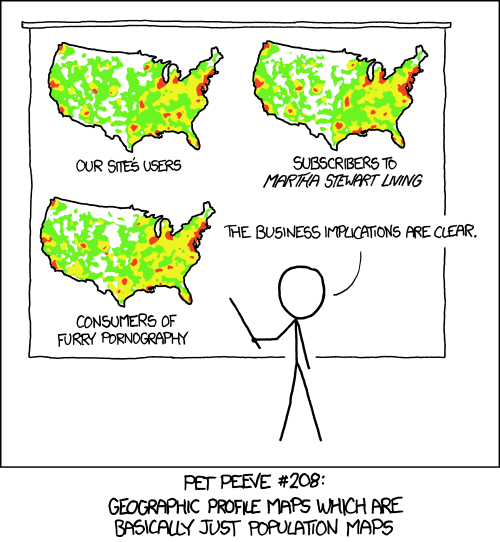
\includegraphics[width=.60\textwidth]{figures/cartoon.png}\end{center}
\end{frame}



\end{document} 